\documentclass[12pt,a4paper]{article}

\usepackage[utf8]{inputenc}
\usepackage[T1]{fontenc}
\usepackage{graphicx}
\usepackage{hyperref}
\usepackage{geometry}
\usepackage{booktabs}
\usepackage{float}
\usepackage{enumitem}
\usepackage{fancyhdr}
\usepackage{xcolor}
\usepackage{listings}
\usepackage{tikz}
\usepackage{colortbl}
\usepackage{mdframed}
\usepackage{fontawesome5}
\usepackage{setspace}

\geometry{margin=1in, headheight=15pt}
\onehalfspacing

\definecolor{primaryblue}{RGB}{26, 115, 232}
\definecolor{darkblue}{RGB}{13, 71, 161}
\definecolor{lightblue}{RGB}{232, 245, 253}
\definecolor{successgreen}{RGB}{46, 125, 50}
\definecolor{lightgray}{RGB}{248, 249, 250}

\hypersetup{colorlinks=true, linkcolor=darkblue, urlcolor=primaryblue}

\lstset{
    basicstyle=\ttfamily\small,
    breaklines=true,
    frame=single,
    backgroundcolor=\color{lightgray},
    numbers=left,
    numberstyle=\tiny\color{gray},
    keywordstyle=\color{primaryblue}\bfseries,
    rulecolor=\color{gray}
}

\newmdenv[
    linecolor=primaryblue,
    backgroundcolor=lightblue,
    linewidth=2pt,
    topline=false,
    rightline=false,
    bottomline=false,
]{highlightblock}

\newmdenv[
    linecolor=successgreen,
    backgroundcolor=successgreen!10,
    linewidth=2pt,
    topline=false,
    rightline=false,
    bottomline=false,
]{successblock}

\pagestyle{fancy}
\fancyhf{}
\fancyhead[L]{\small\color{gray}Individual Contribution Report}
\fancyhead[R]{\small\color{darkblue}\textbf{Anshul Yadav}}
\fancyfoot[C]{\thepage}
\renewcommand{\headrulewidth}{0.5pt}
\renewcommand{\footrulewidth}{0.5pt}

\begin{document}

%========================================
% TITLE PAGE
%========================================
\begin{titlepage}
    \centering
    \vspace*{2cm}
    
    {\Large\color{gray} INDIVIDUAL CONTRIBUTION REPORT\\[0.3cm]}
    
    \rule{0.8\textwidth}{1pt}\\[0.5cm]
    
    {\Huge\bfseries\color{darkblue} Anshul Yadav\\[0.5cm]}
    
    \rule{0.8\textwidth}{1pt}\\[1cm]
    
    {\Large\textit{Garbage Classifier for Waste Management}\\[0.3cm]}
    {\large AI-Powered Garbage Segmentation System\\[1.5cm]}
    
    \begin{tikzpicture}
        \node[draw=primaryblue, fill=lightblue, rounded corners=10pt, minimum width=8cm, minimum height=3cm, align=center] {
            \textbf{\large Primary Roles}\\[0.3cm]
            \faIcon{project-diagram} System Integration\\
            \faIcon{code-branch} Pipeline Development\\
            \faIcon{vial} Testing
        };
    \end{tikzpicture}
    
    \vfill
    
    {\large
    \textbf{BTech (Hons.) CSE - Artificial Intelligence}\\
    5th Semester | Group 09\\[0.5cm]
    University Teaching Department (UTD)\\
    CSVTU, Bhilai\\[0.5cm]
    \textbf{December 2025}
    }
    
\end{titlepage}

\tableofcontents
\newpage

%========================================
% SECTION 1: ROLE OVERVIEW
%========================================
\section{Role Overview}

\begin{highlightblock}
\textbf{\faIcon{user-tag} Assigned Responsibilities:}
\begin{itemize}[leftmargin=*]
    \item[\faIcon{project-diagram}] \textbf{System Integration} — Connecting all components
    \item[\faIcon{code-branch}] \textbf{Pipeline Development} — End-to-end inference flow
    \item[\faIcon{vial}] \textbf{Testing} — Integration and functional testing
\end{itemize}
\end{highlightblock}

%========================================
% SECTION 2: SYSTEM INTEGRATION
%========================================
\section{System Integration}

\subsection{Component Integration}

Integrated the following system modules:

\begin{center}
\begin{tikzpicture}[
    node distance=0.6cm,
    box/.style={rectangle, draw=darkblue, fill=lightblue, minimum width=3cm, minimum height=0.8cm, align=center, rounded corners, font=\small}
]
    \node[box] (preprocess) {\faIcon{magic} Preprocessing};
    \node[box, right=of preprocess] (model) {\faIcon{brain} YOLOv8};
    \node[box, right=of model] (viz) {\faIcon{chart-pie} Visualization};
    \node[box, right=of viz] (ui) {\faIcon{desktop} Gradio UI};
    
    \draw[->, thick, darkblue] (preprocess) -- (model);
    \draw[->, thick, darkblue] (model) -- (viz);
    \draw[->, thick, darkblue] (viz) -- (ui);
\end{tikzpicture}
\end{center}

\subsection{Package Structure}

\begin{lstlisting}[caption=Module Organization]
models/
|-- __init__.py          
|-- yolo_segmentation.py   # Core model
|-- gradio_app.py          # Web interface
|-- inference.py           # Unified pipeline
|-- utils/
    |-- preprocessing.py   # Image enhancement
    |-- visualization.py   # Charts & masks
\end{lstlisting}

\subsection{Integration Pipeline Code}

\begin{lstlisting}[language=Python, caption=Unified Pipeline]
class GarbageDetectionPipeline:
    def __init__(self, use_enhancement=True):
        self.segmentor = GarbageSegmentor()
        self.use_enhancement = use_enhancement
    
    def process(self, image, confidence=0.25):
        # Step 1: Preprocess
        if self.use_enhancement:
            image = auto_brightness(image)
            image = enhance_image(image)
        
        # Step 2: Inference
        self.segmentor.confidence_threshold = confidence
        results = self.segmentor.segment(image)
        
        # Step 3: Visualize
        annotated = self.segmentor.visualize(results)
        
        # Step 4: Statistics
        class_counts = self._count_classes(results)
        pie_chart = create_pie_chart(class_counts)
        
        return annotated, pie_chart, class_counts
\end{lstlisting}

%========================================
% SECTION 3: TESTING
%========================================
\section{Testing}

\subsection{Integration Test Results}

\begin{table}[H]
    \centering
    \caption{Test Cases Executed}
    \rowcolors{2}{lightgray}{white}
    \begin{tabular}{@{}lcc@{}}
        \toprule
        \rowcolor{darkblue}
        \textcolor{white}{\textbf{Test Case}} & \textcolor{white}{\textbf{Status}} & \textcolor{white}{\textbf{Result}} \\
        \midrule
        Single image detection & \textcolor{successgreen}{\faIcon{check}} & Pass \\
        Multiple objects per image & \textcolor{successgreen}{\faIcon{check}} & Pass \\
        Empty image handling & \textcolor{successgreen}{\faIcon{check}} & Graceful \\
        Invalid input handling & \textcolor{successgreen}{\faIcon{check}} & Error msg \\
        Enhancement toggle & \textcolor{successgreen}{\faIcon{check}} & Pass \\
        Confidence threshold & \textcolor{successgreen}{\faIcon{check}} & Pass \\
        UI component rendering & \textcolor{successgreen}{\faIcon{check}} & Pass \\
        \bottomrule
    \end{tabular}
\end{table}

\subsection{Error Handling}

\begin{lstlisting}[language=Python, caption=Robust Error Handling]
def safe_segment(self, image):
    """Segment with error handling."""
    try:
        if image is None:
            return None, "No image provided"
        
        results = self.model.predict(image)
        
        if results[0].masks is None:
            return image, "No objects detected"
        
        return self.visualize(results), "Success"
        
    except Exception as e:
        logging.error(f"Error: {e}")
        return None, f"Error: {str(e)}"
\end{lstlisting}

%========================================
% SECTION 4: ACHIEVEMENTS
%========================================
\section{Technical Achievements}

\begin{successblock}
\textbf{\faIcon{trophy} Key Accomplishments:}
\begin{itemize}[leftmargin=*, label=\faIcon{star}]
    \item Successfully integrated 4 major system components
    \item Developed robust error handling mechanisms
    \item Created unified, modular inference pipeline
    \item Ensured seamless data flow between modules
    \item Conducted comprehensive testing suite
\end{itemize}
\end{successblock}

%========================================
% SECTION 5: SKILLS
%========================================
\section{Skills Demonstrated}

\begin{table}[H]
    \centering
    \rowcolors{2}{lightgray}{white}
    \begin{tabular}{@{}ll@{}}
        \toprule
        \rowcolor{darkblue}
        \textcolor{white}{\textbf{Category}} & \textcolor{white}{\textbf{Skills}} \\
        \midrule
        Architecture & System integration, modular design \\
        Python & Package development, OOP \\
        Quality & Error handling, logging \\
        Testing & Integration testing, QA \\
        \bottomrule
    \end{tabular}
\end{table}

\end{document}
